%%%%%%%%%%%%%%%%%%%%%%%%%%%% Document Class %%%%%%%%%%%%%%%%%%%%%%%%%%%% 
\documentclass{article} % use larger type; default would be 10pt

%%%%%%%%%%%%%%%%%%%%%%%%%%%% PACKAGES TO USE %%%%%%%%%%%%%%%%%%%%%%%%%%%%
%%%%% Page Style %%%%%
\usepackage[margin=1.0in]{geometry}            	% setting the side margins to be ______ inches
\usepackage{fancyhdr}                             		% used to better a custom footer with names/classes/total pages/...
\usepackage{lastpage}                                    	% used to calculate the total page number
%%%%% Functionality %%%%%
\usepackage{enumerate}                                	% making lists       
\usepackage{amsmath}                                   	% includes some math equation functions
\usepackage{graphicx }                                   	% including figures
%\usepackage{sidecap}                                      	% side captions on figures instead of below captions
%%%%% Formatting %%%%%
\usepackage[labelfont=bf]{caption}                  	% setting caption labels to be bold (Table ##, Figure ##)
\usepackage{longtable}					% allows tables that are longer than a single page
\usepackage[font={small,it}]{caption}			% sets captions font to be small italics
\setlength{\belowcaptionskip}{-10pt}                	% removes the extra spacing after captions
\usepackage{color}                                    		% allows one to specify the color of a set of font
\usepackage[section]{placeins}           		% Only allows figures/tables/equations after they are called in line with text
%%%%% Bibliography %%%%% 
\usepackage{cite}                                            	% including the citation package	
\usepackage{natbib}                                        	% used in combination with \setlength to remove the extra spacing in the bibliography
\setlength{\bibsep}{0.0pt}                                	% used in combination with natbib to remove the extra spacing in the bibliography

%%%%%%%%%%%%%%%%%%%%%%%%%%%% Document Title %%%%%%%%%%%%%%%%%%%%%%%%%%%%
\title{Water Vapor Dial Labview Software}
\author{Robert Stillwell}    

%%%%%%%%%%%%%%%%%%%%%%%%%%% Setting the Footer %%%%%%%%%%%%%%%%%%%%%%%%%%%%
\pagestyle{fancy}
\renewcommand{\headrulewidth}{0pt}\lhead{} \chead{} \rhead{}
\lfoot{\sc Stillwell} \cfoot{\normalsize \thepage\ of \pageref{LastPage}} \rfoot{\sc WV DIAL Labview}
%%%%%%%%%%%%%%%%%%%%%%%%%%% Begin Title Page %%%%%%%%%%%%%%%%%%%%%%%%%%%%
\begin{document}                    
\begin{center}
{\sc \LARGE Water Vapor Dial Labview Software} \\
\vspace{0.25in}
{\sc \Large Robert Stillwell\\}
\vspace{0.5in}
{\large NCAR
\\Advanced Study Program
\\ \today}
\end{center}
\vspace{0.5in}
\thispagestyle{empty}

%%%%%%%%%%%%%%%%%%%%%%%%%%% Begin Content Page %%%%%%%%%%%%%%%%%%%%%%%%%%%
\newpage                               	% Making a page break to start the table of contents
\tableofcontents                     	% Making a table of contents
\thispagestyle{empty}		% Removing page number from page
\newpage      				% Making a page break to start of a document
\setcounter{page}{1}            	% Starting page counting here

%%%%%%%%%%%%%%%%%%%%%%%%%%%%%%%%%%%%%%%%%%%%%%%%%%%%%%%%%%%%%%%%%



\section{Acronyms}

\begin{itemize}
\item{DB HSRL: Diode Based High Spectral Resolution Lidar}
\item{MCS: Multi-Channel Scaler}
\item{T DIAL: Temperature Differential Absorption Lidar}
\item{WV DIAL: Water Vapor Differential Absorption Lidar}
\end{itemize}
\newpage    



\section{Nomenclature}

%\begin{itemize}
%\item{Back Panel:\\}
%The portion of the LabVIEW program which contains the wiring diagram and code. 
%\item{Cluster:\\}
%A set of variables saved together in a data structure.
%\item{Control:\\}
%A LabVIEW object which accepts user input and is set before or at runtime. The program can also set this value through a local variable or property node.
%\item{Front Panel:\\}
%The portion of the LabVIEW program which contains user interface and data display. 
%\item{Idle:\\}
%Using a state machine structure, the idle condition is what occurs in the absence of user input after a finite waiting time. In this case, the idle structure performs most typical lidar operations including checking on the data acquisition and reading data.
%\item{Indicator:\\}
%A LabVIEW object which can not be set by the sure at runtime. If the value is set by the user before runtime, the value is overwritten by the program. The program can set this value through a direct call, a local variable, or property node.
%\item{Type Definition:\\}
%A predefined ring loop which can not be redefined without changing the definition itself. This is a way of fixing commonly used terms (like loop stages) such that they can be controlled all at once. 
%\end{itemize}
\newpage    




\chapter{Design}
\label{CH-Design}

\section{Overall Concept}

The design goals for the labview architecture are as follows:

\begin{enumerate}
  \item{Improved fault tolerance}
  \item{Improved data quality \& collection uptime}
  \item{Algoritm isolation for testing and run-time stability}
  \item{Expandable}
  \item{Flexibility to accommodate hardware configuration changes}  \item{Intuitive to new users}
\end{enumerate}

To accomplish these goals, the following concept is proposed. Small individual programs (children) are written to control conceptually seperate processes which interact with the WV DIAL hardware in various ways. In general no more than one child will interact with one piece of hardware to ensure that hardware faults are isolated. These children can run in parallel with proper synchronization and communication via their queues. If one child needs to talk to another it can open that child's queue and add an element onto it. A main container is used to call collections of children programs to accomplish various tasks, and open the necessary children automatically. These sub-functions are all called by the main function based on configure files that correspond to buttons on the main panel. The operational setups that are called by the main function are:

\begin{enumerate}
\item{Warm up sub-function that brings all hardware to operational status. This includes things like warming the lasers and warming the etalons, which needs to be done before high quality data can be taken.}
\item{Main operations sub-function that performs all the mission critical hardware communication during data collection.}
\item{A template sub function which brings up an empty child with minimal functionality.}
\item{Switches sub-function which tests our ability to control the switches.}
\item{Temp. Scan sub-function which sweeps through temperatures to test the lasers.}
\item{Testing sub-functions for individusal controls to check operational status of hardware pieces such as the wavemeter (laser locking), the MCS operation, or the weather station.}
\end{enumerate}

This creates a 3 tiered structure: 1) Main function that opens sub-functions, 2) sub-functions that organize and manage children, and 3) children that actually set and control the state of each individual hardware piece. This creates a natural hierarchy that is predefined. New users unfamiliar with the operation of WV DIAL do not need to know how to control each piece individually but rather are guided through operation. Testing new hardware does not require complete integration with an all in one solution like is currently available, but can be built and tested independantly of the operations of the rest of the DIAL unit. This isolation creates fault tolerance because if one child fails, others are not waiting on that task and data collection for other children can continue unimpeded. Finally, knowledge of the hardware configuration is only needed at the higher levels (the main function and sub-functions) and can be more easily defined than a single all in one program. 





\section{Back Panel Design}\label{Sec:BPDesign}

A template was made to standardize all labview control for WV DIAL. The design is to use queues to execute commands. This allows for an intentional bottleneck of execution such that user and automatically generated commands can not be executed out of order and there are a minimum of changes that need to be made to accommodate new hardware. The automatically generated and user generated commands are in the form of a string that is delimitated by an ``\_". The main loop cases are:
\begin{enumerate}
\item{Configure}
\begin{enumerate}
\item{Reads default state out of the configure file}
\item{Sets the value of all available controls per the configure file}
\item{Sets the function visibility based on control settings like RunAsChild and permissions settings}
\end{enumerate}
\item{Initialize}
\begin{enumerate}
\item{Communicate the initial state of the labview controls to the hardware or vice versa as appropriate}
\item{Create needed file folders for data saving}
\end{enumerate}
\item{Idle}
\begin{enumerate}
\item{Performs baseline commands needed to keep program running}
\item{Waits for user commands to change the state of the system}
\item{Allows for raw data visualization as appropriate}
\end{enumerate}
\item{Error Handler}
\begin{enumerate}
\item{Records all errors in an error log for debugging}
\item{Attempts recovery procedure if the error is recognized}
\item{Alerts the user if error are time sensitive and/or mission critical}
\end{enumerate}
\item{Commanded Exit}
\begin{enumerate}
\item{Performs necessary steps to shutdown hardware that are specific to being told to shut down (only accessible in RunAsChild mode)}
\end{enumerate}
\item{Exit}
\begin{enumerate}
\item{Performs necessary steps to shutdown hardware that are general to RunAsChild or not}
\item{Makes all hidden variables visible again for coding}
\end{enumerate}
\end{enumerate}


\begin{figure}[!ht]\centering
\includegraphics[height=3in]{Figures/MainVITemplateBackPanel}
\caption{A picture of the idle loop stage of the VI template child.}
\label{Fig:VITemplateBP}
\end{figure}

\subsection{The Command and Response Queues}

We have two queues, Command and Response. The command queue is meant to hold user inputs and to process those serially, changing the state of operations. The response queue is meant to hold final data products meant to be written to disk and/or displayed to the screen. The names of these queues is very important. If two queues are running in seperate children with the same name both children will be attempting to put information onto the queues and removing information off of the queues at the same time. When unintended this will cause significant problems in operations. However, this behaviour can be used to facilitate communications between children without the use of global variables and is used to elimiate race conditions that global variables can have. The most prominent example of this usage is with the queue for advanced visualization which is called by different children to communicate the nessicary information to compute and display derived fields.  

\subsection{The Idle Loop}

In the idle loop shown in Figure~\ref{Fig:VITemplateBP}, 4 while loops run. The idle loop is executing commands that are needed to maintain communication with the main function and is used to automatically control the hardware. The user input loop is waiting for user commands and adding them to the command queue. The execution loop is processing elements off of the command queue and taking action within the Interpret Commands and Responses subVI. Critically, this function is called in re-entrant execution mode as it is copied in all functions. Lastly the visualization loop which is used to process hardware responses from the response queue, save the results to disk, and to print the results to the screen. 

\subsection{Run as Stand Alone}

The multiple function concept requires one functional distinction. One concept is to run each piece manually, and another is to have a main function run each piece automatically, refered to as running in stand alone mode or running as child, respectively.   

A template for the individual control elements is given in Figure \ref{Fig:VITemplate}. There are 3 main boxes, the first is in the top left (labeled as ``Place Commands Here") for all of the user controls and everything the user needs to see. This will be different for each control. Within that box is a smaller box that would be the same for all controls that help locate the current status of the queue. The second box directly below would appear if the control were running as a stand alone but be hidden if the control were running as child. This really only needs to be in one place and is constant for all functions. The final box to the right is always hidden but is the storage place for all hidden variables that need to be defined but that the user does not need to see. 

\begin{figure}[!ht]\centering
\includegraphics[height=3in]{Figures/MainVITemplate}
\caption{The front panel of the main VI template. The software at runtime will hide the unnecessary controls and shrink the front panel window the the appropriate size indicated by the outer boxes. If the VI is run as a child (called from a higher VI) the Global Buttons disappear. }\label{Fig:VITemplate}
\end{figure}

Each child is stored in its own library. They are WeatherStation.llb, WavelengthLocking.llb, QuantCompControl.llb, NetCDFWriter.llb, MCS\_NCAR.llb, MCSControls\_NCAR.llb, Logbook.llb, IndividualChildControl.llb, and AdvancedVis.llb. WVDIAL\_Main.vi is the definition of the main container and the main VI to start the software. The library ContainerResources.llb is used to support the main contianer. Futhermore there are some VI's which are useful to more than one child and are stored in SharedResorces.llb. Some LabView objects are complex and need to be passed through several VIs, so type definitions are used to communicate the structure of those complex structures. Those TypeDefs are stored in TypeDefinitions.llb. 

This standardization via the template is not critical for running all VIs as stand alone, however, the solution for running all the VIs as children in parallel does. 

\subsection{Run as Child}

For the case that these individual controls are to be run automatically in parallel, an organizational problem arises. Assuming the code running the individual controls as children knows what functions to open and in what order, it is still possible that a user accidentally closes one function or a mess of VIs appears. To solve this, all front panels of the VIs running are projected into a single container seperated by a tabular control. The container itself has very little code running but is just there to contain all of the sub-VIs. This container is shown in Figure \ref{Fig:VIContainer}.

\begin{figure}[!ht]\centering
\includegraphics[height=3in]{Figures/MainVIContainer}
\caption{The front panel of the main VI container. If multiple VIs are called and run simultaneously, their front panels are projected into the main container to allow for a simple control for the user but also allows maximum flexibility in VI execution.}\label{Fig:VIContainer}
\end{figure}

In this case, the controls that are common to all VIs, in the bottom box of Figure \ref{Fig:VITemplate}, are collected and included only once. Because the front panels of all VIs are to be projected into a single container, the front panel sizes of all VIs should be of a standard size otherwise the container would not simplify much. The container itself  is simply a set of sub-panels that can each hold a single VI. The maximum number of VIs needed can be written if fewer are required, and the main program simply hides unused sub-panels. 

\subsection{Configure Files}
Instead of using default variables in Labview, the default configuration for each sub-program will be stored in a configuration file. This ensures that operational hardware configurations are decoupled from any software upgrades or changes. Additionally, it makes it always possible to return the software to a known pre-set operational state and makes it more difficult for users to unknowingly modify the hardware's initial state. The configure files are version controlled via Git to track changes over time. An example of a configure file is given in Figure \ref{Fig:ConfigureFile}. 

\begin{figure}[!ht]\centering
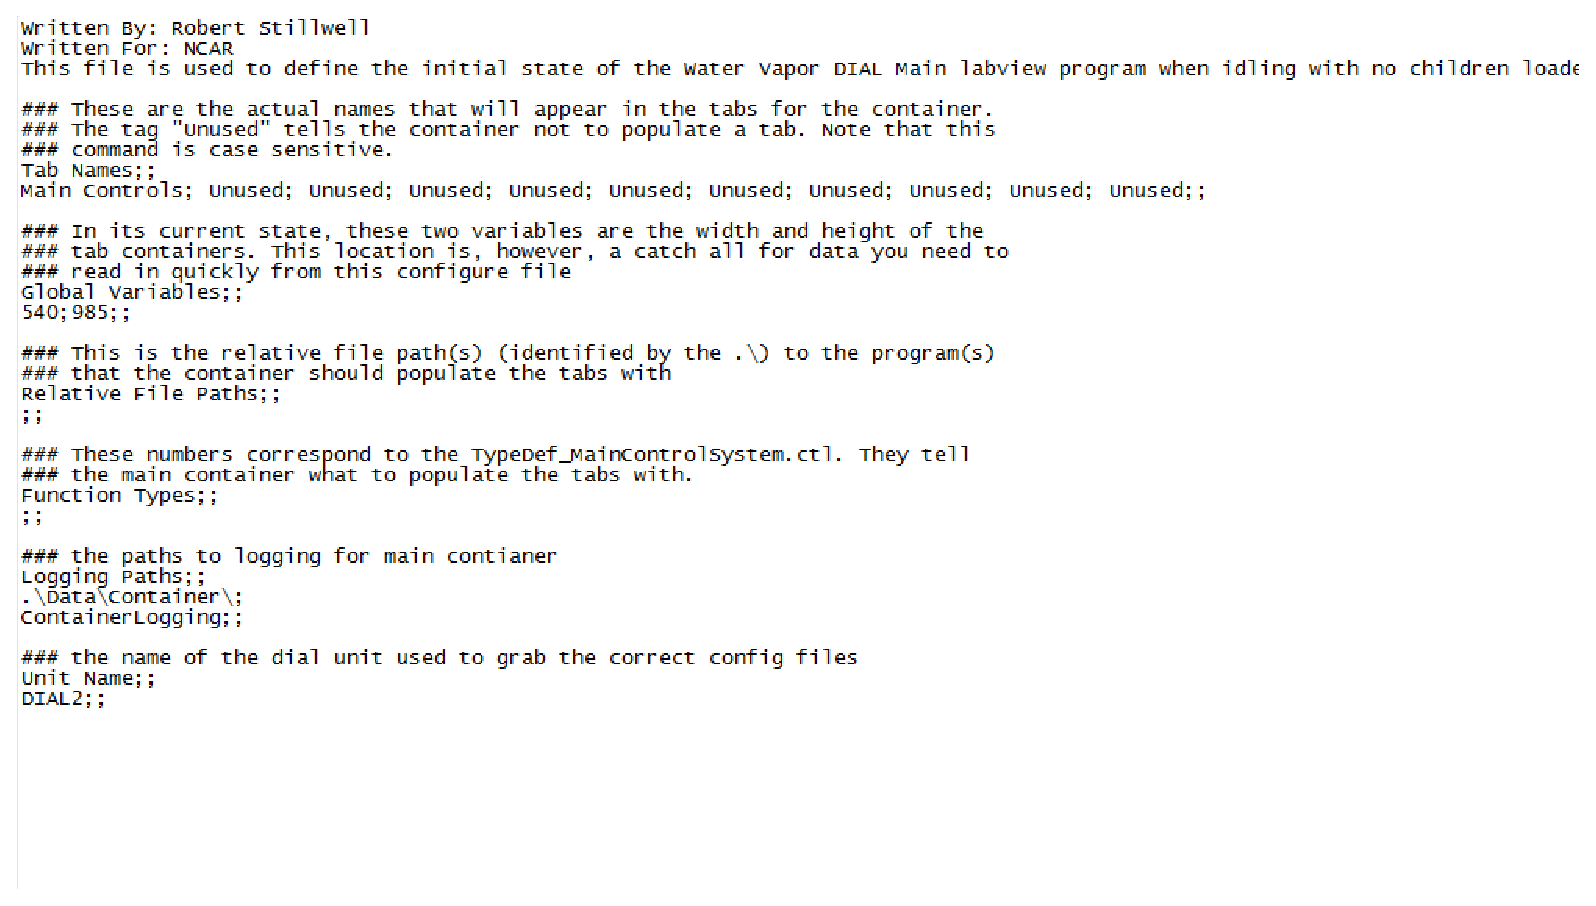
\includegraphics[height=3in]{Figures/ConfigureFileExample}
\caption{An example of the structure of a configure file. Variables are identified by a single name followed by two semi-colons. The next line has the required values delimitated by a single semi-colon with the end of line denoted by a double semi-colon.}\label{Fig:ConfigureFile}
\end{figure}

\subsection{Log Files}

Log files are to be kept to help track the status of WV DIAL and to help debug any anomalous states. The logs to be kept are:

\begin{enumerate}
\item{Operations Logs: Describes when the system starts and stops and any user defined changes}
\item{Warning logs: These indicate failures in operations which does not inhibit mission critical functionality.}
\item{Error logs: These indicate failures in mission ciritical functionality and must be addressed imediatly.}
\end{enumerate}

\subsection{Type Definitions}

One of the unfortunate features of labview occurs when trying to modify the contents of a complicated structure. For example, if you initially make a cluster to define the state of a single laser and wish to add a piece to that structure, labview will show each connected wire as broken throughout the entire program. To solve this, labview allows the user to define structure types and to link the controls on all panels directly to that definition. This allows the user to make a change in a single place and have all variables referenced to that place change at the same time. 

This type definition is widely used for controls. It requires an extra step to make the definition then load it into the program much like defining a global variable but it makes updating and maintaining the code simpler and cleaner. 






\section{Children}\label{Sec:Children}

Each child was created to seperate and isolate funcitonality. These children were built based off of the template, but several differ from that design for specific reasons. Listed below are descriptions of how the children used for main data collection differ from the template design. 

WeatherStation.llb contains files needed for operation of the weather station. It is perhaps the simplist of all the children and simply sticks to the design of the template to do so.  

MCS\_NCAR.llb and MCSControls\_NCAR.llb when taken together form the data acquasition system and controls for the MCS. Because of the timing sensitivity and mission critical nature of the photon counting data, the MCS\_NCAR child has an additional loop whose sole responsibility is to monitor the UDP port communications and never allow itself to get interupted from that goal. This means it has an additional UDP loop thread dedicated to monitoring the UDP port which is seperated from the normal idle loop. Furthermore MCSControls\_NCAR is used to seperate the controls from the hardware communication a layer further, so as to add an extra layer of safty to ensure that users fiddling with controls may be isolated from the reading of the UDP port. To this end any failure in the MCSControls will not interupt the collection of photon counting data. 

WavelengthLocking.llb ********** - Robert will have to fill this one in more detail, as he wrote this and will have more insight into its operations - **********

AdvancedVis.llb seems at first to be straightforward. It pulls information from the MCS, the weather station, etc... in order to display composite data fields. This communication method however must remain true to the goals of isolating functionality and ensure that any failures in one child do not leak through to others. The way we do this (which is also done between MCS\_NCAR and MCSControls\_NCAR) is to establish queue communications where a child may add instructions onto the queue of another child. This requires the name of the queue in order to add to it, and as such the names of the queues should not be changed in order to maintain these avenues of communication. Advanced visualization gathers data from several sources so this method of communication is quite useful in this case. 

IndividualChildControl.llb contains both the housekeeping child and the UPS child. Both of these children stick to the design of the original template quite closely. The UPS does, however, have routines for sending email messages in the case of loss of power to the unit so power outages can be addressed as quickly as possible. 

NetCDFWriter.llb acts as a data compiler. It takes the raw txt and bin files written by each of the other data writing children and converts them into raw NetCDF files and finally into the final data product which is a merged CFRadial file. LabView does not have the capabilities to write NetCDF files directly, so for this purpose a python subroutine is called in order to deliver the final data products. These data products are described in Chapter~\ref{CH-Data}.




\section{Individual Element Controls}
The proposed software update parses the main hardware control function into sub-functions. These sub-functions serve to control individual elements of the WVDIAL, serve as simplified routines to warm up elements of the WVDIAL, or are to test out specific functionality in isolation of the rest of the unit. 

\subsection{MCS}\label{Sec:MCSSubFunction}

A sub-function that brings up two children. One does the communications via UDP to read the MCS, while the other is a set of controls to change the state of the MCS. These were split into two functions in order to prioritize the UDP communication so photon counting data was always running without interuption, and so that while the child was reading the UDP port the controls would continue to feel responsive. In a previous version of the MCS software putting the UDP communications in the same VI as the controls would lead to delays in the responsivness of the front panel due to the translation from a series of controls into a 32 bit hex word and back that was needed for MCS communications. 

\subsection{Weather Station}\label{Sec:WSSubFunction}

A sub-function that brings up the weather station child to monitor surface level temperature, pressure, relative humidity, and absolute humidity. 

\subsection{Laser Locking}\label{Sec:LLSubFunction}

A sub-function that brings up the laser locking routines that controls laser wavelengths and the etalons. 

\subsection{Housekeeping}\label{Sec:HousekeepingSubFunction}

A sub-function that brings up one child whose responsibility is to relay information about the temperature of the container. Thermocouples are placed within the container in various positions which can be specified for writing into the data in the Configure\_WVDIALPythonNetCDFHeader.txt. This is primarily to help ensure that the climate control for the unit is functioning properly. 

\subsection{UPS}\label{Sec:UPSSubFunction}

A sub-function that calls the UPS child to monitor the state of the UPS Battery and power to the unit. The UPS child has a subroutine to automatically send out an email when the UPS Battery gets too low. 

\subsection{HSRL Oven}\label{Sec:HSRLOvenSubFunction}

A sub-function that warms up the HSRL. This is not currently built, but the button on the front panel is there for the addition of the feature in the future. 

\subsection{Wavemeter}\label{Sec:WavemeterSubFunction}

A sub-function that brings up the wavemeter to read the wavelengths of the lasers. 

\subsection{Thor 8000}\label{Sec:T8000SubFunction}

A sub-function that controls the Thor 8000 laser diode current control module. 

\subsection{Quantum Composer}\label{Sec:QCSubFunction}

A sub-function that controls the Quantum Composer timing unit. For the Relampago release the only functionality is to write, the read function does not work. When writing to the QC you may have to click through a couple pop ups in order to sucessfully set the state of the QC. 

\subsection{Power Switches}\label{Sec:PowSwitchSubFunction}

A sub-function that controls the power switches.

\subsection{NetCDF}\label{Sec:NetCDFSubFunction}

A sub-function that brings up the NetCDF writer for reprocessing of data files.





\section{Sub-Functions and Calling}

All of the individual controls are collected into a single container to run more complicated tasks. For example, the main operation of WV DIAL at full capability would require simultaneous control of the MCS, weather station, laser locking, etc.... The labview code runs the children responsible for each of these tasks and stores them in a single container. 

If a single VI fails, the other sub-functions are not affected by it. Its data would, however, be missing from the final data product. For example, if the weather station communication failed, that data would be missing but it is not mission critical to have at all times. When its service could be restored, the weather station data stream would be restored without interuption of other services. Details of how that data appears is outlined in Chapter~\ref{CH-Data}.

\newpage 



\chapter{Data}
\label{CH-Data}

\section{Raw Data Output}
\label{Sec-DATAOutput}

\subsection{Raw File Naming Convention}
 A naming convention for the files written is proposed as:

\begin{enumerate}
\item{MCS Data: NCARWVDIAL\#\#\#\_MCS\_YYYYMMDD\_HHMMSS.cdf where \#\#\# is the number of the instrument, YYYYMMDD is the year, month and day of the file creation, and HHMMSS is the hour, minute, and second of file creation.}
\item{Weather Station Data: NCARWVDIAL\#\#\#\_WeatherStation\_YYYYMMDD\_HHMMSS.cdf where \#\#\# is the number of the instrument, YYYYMMDD is the year, month and day of the file creation, and HHMMSS is the hour, minute, and second of file creation.}
\item{Transmitter Housekeeping Data: NCARWVDIAL\#\#\#\_HousekeepingTx\_YYYYMMDD\_HHMMSS.cdf where \#\#\# is the number of the instrument, YYYYMMDD is the year, month and day of the file creation, and HHMMSS is the hour, minute, and second of file creation.}
\item{Receiver Housekeeping Data: NCARWVDIAL\#\#\#\_HousekeepingRx\_YYYYMMDD\_HHMMSS.cdf where \#\#\# is the number of the instrument, YYYYMMDD is the year, month and day of the file creation, and HHMMSS is the hour, minute, and second of file creation.}
\end{enumerate}

\subsection{Main Data Product Changes}

The main changes from previous architecture and how those changes help accomplish design goals are listed below.
\begin{enumerate}
\item{NetCDF file types instead of binary files.}
	\begin{enumerate}
		\item{Pros:
			\begin{enumerate}
				\item{Expandable and customizable to different hardware configurations or improvements.}
				\item{Can be easily converted to have outputs to mirror the GV HSRL or in CFRadial format.}
				\item{Can be easily read and understood by non-NCAR personnel lacking knowledge of binary format.}
				\end{enumerate}
		}
		\item{Cons:
			\begin{enumerate}
				\item{Requires a change to the post processing ingest code.}
				\item{As far as I can tell, only allows for a single unlimited variable making it not possible to stream data at different cadences to the same file efficiently.}
				\end{enumerate}
		}
	\end{enumerate}
\item{Multiple files containing data instead of a single file per hour. The plan is to split the hourly files into a file containing: all photon counts and power measurements (measurements from the MCS), weather station data, laser housekeeping and locking data, and receiver housekeeping data. Additionally, on restart, a new netCDF file will be created instead of reopening the current hour's file.}
	\begin{enumerate}
		\item{Pros:
			\begin{enumerate}
				\item{Data for WV DIAL can be taken at different cadences. Though the current architecture can accommodate all data being taken at the same cadence, it is not necessary. There is no physical reason to take weather station data at 2 second resolution for example. By allowing multiple files, data can be taken at physically meaningful resolution and recombined in post processing.}
				\item{Shrinks data files: Removing the requirement to take data at the same resolution removes redundant measurements.}
				\item{Data transfer flexibility: Over limited data transfer links, such as a cell modem or at bandwidth limited sites, the most critical data can be identified and transferred while still saving all data for post processing.}
				\item{Hardware changes or major changes requiring Labview shutdown can be easily tracked by file header information.}
			\end{enumerate}
		}
		\item{Cons:
			\begin{enumerate}
				\item{Data requires recombination to a single time grid in post processing.}
				\item{The proposed split may require multiple VIs talk to the same hardware. This will require an access check before writing commands to make sure that two commands are not sent simultaneously that confuses the hardware.}
			\end{enumerate}
		}
	\end{enumerate}
\item{Writing photon counting data at native resolution regardless of the state of the transmitter or receiver. This requires status bits being recorded instead of only recording data when all status bits indicate good data.}
	\begin{enumerate}
		\item{Pros:
			\begin{enumerate}
				\item{Data is not missed for one laser while other lasers are locking.}
				\item{Data collection decoupled from all other data makes sure you are not loosing data for a reason other than MCS failure. For example, if the HSRL laser turns off, the system will be stuck trying to lock a laser it can't find. Meanwhile, WV data is lost that is not necessarily bad. }
			\end{enumerate}
		}
		\item{Cons:
			\begin{enumerate}
				\item{Data file must now include status flags that were not needed before.}
			\end{enumerate}
		}
	\end{enumerate}
%\item{C}
%	\begin{enumerate}
%		\item{Pros:
%			\begin{enumerate}
%				\item{1.}
%				\item{2.}
%				\item{3.}
%			\end{enumerate}
%		}
%		\item{Cons:
%			\begin{enumerate}
%				\item{1.}
%				\item{2.}
%			\end{enumerate}
%		}
%	\end{enumerate}
\end{enumerate}


\newpage




\section{Raw Data Ingest and Mating with Python Scripts}


Steps of unpacking a single day of data:
\begin{enumerate}
	\item{Loop over hourly folders (I prefer to dump all data into a single daily directory but that is a convenience not a necessity)}
	\begin{enumerate}
		\item{Loop over hourly file types (more that one of each type can be written if the labview is started more than once in a single hour or restarted)}
			\begin{enumerate}
				\item{Check if particular file contains data (by checking for zero-valued dimensions)}
				\item{Loading raw photon count data}
				\item{Loading laser housekeeping data}
				\item{Loading weather station data}
				\item{Loading the operational parameters of the system and time stamps for each file type}
			\end{enumerate}
		\item{Interpolate slower data to highest cadence data (likely housekeeping and weather station data to photon count time grid)}
		\item{Collect all data into a single daily file with a single time dimension}
		\item{Fill in missing data in time (if any time gaps exist) with nan values}
		\item{Combine laser locking, receiver temperature, and all other data flags and create a single quality control flag: (Use Data, Data Warning, or Don't Use)}
	\end{enumerate}
\end{enumerate}


\newpage




\section{Raw Data Ingest and Mating with Python Scripts}


Steps of unpacking a single day of data:
\begin{enumerate}
	\item{Loop over hourly folders (I prefer to dump all data into a single daily directory but that is a convenience not a necessity)}
	\begin{enumerate}
		\item{Loop over hourly file types (more that one of each type can be written if the labview is started more than once in a single hour or restarted)}
			\begin{enumerate}
				\item{Check if particular file contains data (by checking for zero-valued dimensions)}
				\item{Loading raw photon count data}
				\item{Loading laser housekeeping data}
				\item{Loading weather station data}
				\item{Loading the operational parameters of the system and time stamps for each file type}
			\end{enumerate}
		\item{Interpolate slower data to highest cadence data (likely housekeeping and weather station data to photon count time grid)}
		\item{Collect all data into a single daily file with a single time dimension}
		\item{Fill in missing data in time (if any time gaps exist) with nan values}
		\item{Combine laser locking, receiver temperature, and all other data flags and create a single quality control flag: (Use Data, Data Warning, or Don't Use)}
	\end{enumerate}
\end{enumerate}


\newpage




\section{Known Issues and How This Proposal Affects Them}

\begin{enumerate}
\item{Data for on and offline wavelengths written in two different files. Matt mentioned this as a possible problem that I believe is linked to the serial nature of laser locking and data collection. By making the two asynchronous and including a laser locking flag instead of waiting for ti to complete, one can read data from the MCS and write data in 2 sets and not 4. Just have to make sure that a file can not be initialized before writing is complete.}
\item{Single errors crash the whole system. This overall design is more fault tolerant. Additionally, error logging will be included in the initial version such that we can record what is crashing the system and come up with systematic ways to deal with it.}
\item{Slow laser locking: This outline is agnostic to the type of locking but can certainly accommodate a new PID or simple integral locking scheme. }
\item{Blue screen of death! The hope is that making each communication a smaller piece allows for easier debugging of the culprit. (NOTE: moving to the new micro form factor computer may have solved this issue, coninuing testing needed to confirm}
\end{enumerate}

\newpage



\chapter{Other Labview Details}
\label{CH-Other}

\section{Front Panel}
\section{Back Panel}

It is easy to forget the Labview standard back panel color coding scheme so It is included here for reference in Table~\ref{Table:BPColorCoding}. 

\begin{table}[h]
\centering
\caption{Labview Standard back panel color coding scheme.}
\begin{tabular}{clc}
\hline\hline
Color	& Type								& Picture														\\
\hline
Blue		& 									& 															\\\hline
		& Integrers							& \includegraphics[height=0.2in]{Figures/ColorCoding_Int}				\\\hline
		& VI or Queue Reference					& \includegraphics[height=0.2in]{Figures/ColorCoding_VIReference}			\\\hline
Green	&									&															\\\hline
		& Boolean								& \includegraphics[height=0.2in]{Figures/ColorCoding_Bool}				\\\hline
		& File Path							& \includegraphics[height=0.2in]{Figures/ColorCoding_FilePath}			\\\hline
		& Error Cluster							& \includegraphics[height=0.2in]{Figures/ColorCoding_Error}				\\\hline
		& Robert's functions	(might like to change this) 	& \includegraphics[height=0.4in]{Figures/ColorCoding_Custom}			\\\hline
Orange	& 									& 															\\\hline
		& Double								& \includegraphics[height=0.2in]{Figures/ColorCoding_Float}				\\\hline
Pink		&									&															\\\hline
		& Cluster								& 
\includegraphics[height=0.2in]{Figures/ColorCoding_Cluster}				\\\hline
		& String								& \includegraphics[height=0.2in]{Figures/ColorCoding_String}				\\\hline
Purple	& Hardware Resource					& \includegraphics[height=0.2in]{Figures/ColorCoding_HardwareReference}	\\\hline
\end{tabular}
\label{Table:BPColorCoding}
\end{table}


%%%%%%%%%%%%%%%%%%%%%%%%%%%%%%%%%%%%%%%%%%%%%%%%%%%%%%%%%%%%%%%%%
\section{Priority Settings}
Because the main structure of the software is based around queues, it is possible to remove elements from a queue before they are executed, put things on top of the queue in front of other commands, or put things at the bottom. Additionally, for performing commands that occur in steps, the queue is an ideal solution for organizing commands. Each of these possibilities is governed by a priority setting. For normal operation, the string commands are added to the bottom of the queue. If that queue is full or has several items in it, a standard command will not take precedent over other commands. The user abort command, for instance, has first priority. This command flushes the queue of current commands and inserts the set of commands to shut the system down.


%%%%%%%%%%%%%%%%%%%%%%%%%%%%%%%%%%%%%%%%%%%%%%%%%%%%%%%%%%%%%%%%%
\section{Password Settings} \label{Sec:Password}

NOTE: This functionality has not been built upon for Relampago, but the back end is in place for it to be added when desired. All commands are currently set up as accessable to all levels of user. 

There are three password levels. They allow various things to happen such as bypassing the hardware warmup cycle or changing laser settings or turning off key components. Each level requires a password then the level permissions are hardwired into the code. When developed a list of password protected actions will be given here where the level is specified as either 1,2, or 3. Permissions on startup will begin at 0, which is recognized as unset. To prevent the user with a lower access level to attempt to use a sensitive command the main programs will set the visibility of certain controls such that they disappear with lower access.

The levels are complete access (or developer access), access to all but the most sensitive features (called administrative access), and general access. The passwords for each level are:

\begin{enumerate}
\item{developer: \%1543Lidar}
\item{administrative: !532Lid@r}
\item{general: SoundAndFury}
\end{enumerate}

Once a password level is recognized, all the privileges of the lower levels comes with the highest. That said, there are two passwords to downgrade access from a higher to a lower level. Note that if one is signed in with developer access and tries to downgrade to general access with the above given password, the password function will maintain the current access level. The two downgrading passwords are for completely unsetting the permissions and going back to general access. The passwords are respectively listed as:

\begin{enumerate}
\item{Clear}
\item{Revert}
\end{enumerate}

All passwords are case sensitive.

There is one way to beat the password protection provided by the visibility and password functions which is possible but not likely. As the main function executes most of the user desired functions by creating and executing string commands, the main way to defeat the password options is to open and directly use the string execution commands. The commands are defaulted to do nothing if not entered exactly correctly but will execute a command if the user types the correct string commands. If for example, the string command is incomplete or the case sensitive commands do not match exactly what the execution function is looking for, an return string will note that the command is unrecognized. 

A list of actions that require passwords and the level required that is proposed is given below.

\begin{longtable}{ccl}
Command				& Level  	& Reason										\\
\hline
example\_command & Level\# & Thing It Does	\\
\hline
\label{Tab:PasswordDetails}\end{longtable}

\newpage




%%%%%%%%%%%%%%%%%%%%%%%%%%% Ending document %%%%%%%%%%%%%%%%%%%%%%%%%%%%
\end{document}
